\documentclass[11pt]{article}
\usepackage{tikz}
\usetikzlibrary{shapes, arrows}
\usepackage[hmargin=1in,vmargin=1in]{geometry}
\usepackage{xcolor}
\usepackage{enumitem} 
\usepackage{wrapfig}
\usepackage{amsmath,amssymb,amsfonts,url,sectsty,framed,tcolorbox,framed}
\newcommand{\pf}{{\bf Proof: }}
\newtheorem{theorem}{Theorem}
\newtheorem{lemma}{Lemma}
\newtheorem{proposition}{Proposition}
\newtheorem{definition}{Definition}  
\newtheorem{remark}{Remark}
\newcommand{\qed}{\hfill \rule{2mm}{2mm}}
\usepackage{fixltx2e}
\usepackage{graphicx}
\newcommand*{\xdash}[1][3em]{\rule[0.5ex]{#1}{0.55pt}}
\begin{document}
	\noindent
	\rule{\textwidth}{1pt}
	\begin{center}
		{\bf [CS304] Introduction to Cryptography and Network Security}
	\end{center}
	Course Instructor: Dr. Dibyendu Roy \hfill Winter 2022-2023\\
	Scribed by : Pallikonda Sai Teja  \hfill Lecture (Week 07)\\
	Student ID : 202011052\\
	\rule{\textwidth}{1pt}
	\section{Advanced Encryption Standard AES}
	\subsection{Shift Rows}
	Shift Rows : \{0, 1\}$^{128}$ $\rightarrow$ \{0, 1\}$^{128}$\vspace{0.2cm}\\
	\begin{tabular}{c | c c c c |}
		0&S\textsubscript{00} & S\textsubscript{01} & S\textsubscript{02} & S\textsubscript{03}\\
		1&S\textsubscript{10} & S\textsubscript{11} & S\textsubscript{12} & S\textsubscript{13}\\
		2&S\textsubscript{20} & S\textsubscript{21} & S\textsubscript{22} & S\textsubscript{23}\\
		3&S\textsubscript{30} & S\textsubscript{31} & S\textsubscript{32} & S\textsubscript{33}
	\end{tabular}\hspace{0.2cm}$\rightarrow$\hspace{0.2cm}
	\begin{tabular}{| c c c c |}
		S\textsubscript{00} & S\textsubscript{01} & S\textsubscript{02} & S\textsubscript{03}\\
		S\textsubscript{11} & S\textsubscript{12} & S\textsubscript{13} & S\textsubscript{10}\\
		S\textsubscript{22} & S\textsubscript{23} & S\textsubscript{20} & S\textsubscript{21}\\
		S\textsubscript{33} & S\textsubscript{30} & S\textsubscript{31} & S\textsubscript{32}
	\end{tabular}
	
	\subsection{Mix Column}
	Mix Column : \{0, 1\}$^{128}$ $\rightarrow$ \{0, 1\}$^{128}$\vspace{0.2cm}\\
	(S\textsubscript{ij})\textsubscript{4x4} $\rightarrow$ (S\textsubscript{ij}$^l$)\textsubscript{4x4}\\
	Consider the column c $\in$ \{0, 1, 2, 3\}\vspace{0.2cm}\\
	column = \begin{tabular}{|c|}
		S\textsubscript{0c}\\
		S\textsubscript{1c}\\
		S\textsubscript{2c}\\
		S\textsubscript{3c}
	\end{tabular}\vspace{0.2cm}\\
	S\textsubscript{ic} = (a\textsubscript{7}a\textsubscript{6}a\textsubscript{5}a\textsubscript{4}a\textsubscript{3}a\textsubscript{2}a\textsubscript{1}a\textsubscript{0})\\
	Polynomial = a\textsubscript{0} + a\textsubscript{1}$x$ + a\textsubscript{2}$x^2$ + ... + a\textsubscript{7}$x^7$\vspace{0.2cm}\\
	\textit{for i= 0 to 3}\\
	\hspace*{1cm}t\textsubscript{i} = Binary to Polynomial(S\textsubscript{ic})\\
	u\textsubscript{0} = [(x $\ast$ t\textsubscript{0}) + (x+1) $\ast$ t\textsubscript{1} + t\textsubscript{2} + t\textsubscript{3}] mod($x^8$ + $x^4$ + $x^3$ + $x$ + 1)\\
	u\textsubscript{1} = [(x $\ast$ t\textsubscript{1}) + (x+1) $\ast$ t\textsubscript{2} + t\textsubscript{3} + t\textsubscript{0}] mod($x^8$ + $x^4$ + $x^3$ + $x$ + 1)\\
	u\textsubscript{2} = [(x $\ast$ t\textsubscript{2}) + (x+1) $\ast$ t\textsubscript{3} + t\textsubscript{0} + t\textsubscript{1}] mod($x^8$ + $x^4$ + $x^3$ + $x$ + 1)\\
	u\textsubscript{3} = [(x $\ast$ t\textsubscript{3}) + (x+1) $\ast$ t\textsubscript{0} + t\textsubscript{1} + t\textsubscript{2}] mod($x^8$ + $x^4$ + $x^3$ + $x$ + 1)\\
	(S\textsubscript{ij}$^l$) = Polynomial to Binary(u\textsubscript{i})\vspace{0.2cm}\\
	\begin{tabular}{|c|}
		S\textsubscript{0c}\\
		S\textsubscript{1c}\\
		S\textsubscript{2c}\\
		S\textsubscript{3c}
	\end{tabular} $\rightarrow$ Mix Column $\rightarrow$ 
	\begin{tabular}{|c|}
		S\textsubscript{0c}$^l$\\
		S\textsubscript{1c}$^l$\\
		S\textsubscript{2c}$^l$\\
		S\textsubscript{3c}$^l$
	\end{tabular}\vspace{0.2cm}\\
	\begin{tabular}{| c c c c |}
		x & x + 1 & 1 & 1\\
		1 & x & x + 1 & 1\\
		1 & 1 & x & x + 1\\
		x + 1 & 1 & 1 & x\\
	\end{tabular} $\ast$
	\begin{tabular}{| c c c c |}
		S\textsubscript{00} & S\textsubscript{01} & S\textsubscript{02} & S\textsubscript{03}\\
		S\textsubscript{10} & S\textsubscript{11} & S\textsubscript{12} & S\textsubscript{13}\\
		S\textsubscript{20} & S\textsubscript{21} & S\textsubscript{22} & S\textsubscript{23}\\
		S\textsubscript{30} & S\textsubscript{31} & S\textsubscript{32} & S\textsubscript{33}
	\end{tabular} mod(x$^8$ + x$^4$ + x$^3$ + x + 1) = (S\textsubscript{ij}$^l$)\textsubscript{4x4}\\
	
	\subsection{Key Scheduling Algorithm of AES-128}
	Input : 128 bit key.\\
	Output : 11 Round Keys, each of length 128 bit.\vspace{0.2cm}\\
	Key = [Key[15], Key[14],.., Key[0]] $\rightarrow$ 16 bytes\\
	We will prepare 44 words which are denoted by w[0], w[1], ..., w[43].\vspace{0.1cm}\\
	$\bullet$ \textit{ROTWORD(B\textsubscript{0}, B\textsubscript{1}, B\textsubscript{2}, B\textsubscript{3}) = (B\textsubscript{1}, B\textsubscript{2}, B\textsubscript{3}, B\textsubscript{0})}\\
	$\bullet$ \textit{SUBWORD(B\textsubscript{0}, B\textsubscript{1}, B\textsubscript{2}, B\textsubscript{3}) = (B\textsubscript{0}$^l$, B\textsubscript{1}$^l$, B\textsubscript{2}$^l$, B\textsubscript{3}$^l$)}\\
	where B\textsubscript{i}$^l$ = SUBBYTE(B\textsubscript{i}) $\forall$ i $\in$ \{0, 1, 2, 3\}\vspace{0.1cm}\\
	$\bullet$ 10 Round Constants (Word)\\
	Rcon[1] = 01000000\\
	Rcon[2] = 02000000\\
	Rcon[3] = 04000000\\
	Rcon[4] = 08000000\\
	Rcon[5] = 10000000\\
	Rcon[6] = 20000000\\
	Rcon[7] = 40000000\\
	Rcon[8] = 80000000\\
	Rcon[9] = 1B000000\\
	Rcon[10] = 36000000\vspace{0.1cm}\\
	for i = 0 to 3\\
	\hspace*{0.8cm}w[i] = (Key[4i], Key[4i+1], Key[4i+2], Key[4i+3])\vspace{0.1cm}\\
	for i = 4 to 43\\
	\hspace*{0.8cm}temp = w[i-1]\\
	\hspace*{0.8cm}if i $\equiv$ 0 mod4\\
	\hspace*{1.3cm}temp = \textit{SUBWORD(ROTWORD}(temp)) $\oplus$ Rcon[i/4]\\
	\hspace*{0.8cm}w[i] = w[i-4] $\oplus$ temp\\
	return (w[0], w[1],..., w[43])\vspace{0.1cm}\\
	Key\textsubscript{1} = w[0] $||$ w[1] $||$ w[2] $||$ w[3]\\
	Key\textsubscript{2} = w[4] $||$ w[5] $||$ w[6] $||$ w[7]\\
	.\\
	.\\
	Key\textsubscript{10} = w[40] $||$ w[41] $||$ w[42] $||$ w[43]
	\subsection{Sub Bytes}
	Subbyte(A) = ?\\
	A = X $||$ Y. Here X is the row number and Y is the column number in Subbyte table. And from subByte table we can find SubByte(A).
	\subsection{Inverse Sub-Bytes}
	SubByte(A) = B\\ 
	Find A given B.\\
	So, Firstly find B inside the table by exhaustive search.\\
	X $\rightarrow$ Row Number.\\
	Y $\rightarrow$ Column Number.\\
	Output = X $||$ Y\\
	A = X $||$ Y
	\subsection{Inverse Shift Row}
	\begin{tabular}{| c c c c |}
		S\textsubscript{00} & S\textsubscript{01} & S\textsubscript{02} & S\textsubscript{03}\\
		S\textsubscript{10} & S\textsubscript{11} & S\textsubscript{12} & S\textsubscript{13}\\
		S\textsubscript{20} & S\textsubscript{21} & S\textsubscript{22} & S\textsubscript{23}\\
		S\textsubscript{30} & S\textsubscript{31} & S\textsubscript{32} & S\textsubscript{33}
	\end{tabular}\hspace{0.2cm}$\rightarrow$\hspace{0.2cm}
	\begin{tabular}{| c c c c |}
		S\textsubscript{00} & S\textsubscript{01} & S\textsubscript{02} & S\textsubscript{03}\\
		S\textsubscript{13} & S\textsubscript{10}&S\textsubscript{11} & S\textsubscript{12}\\
		S\textsubscript{22}&S\textsubscript{23} & S\textsubscript{20} & S\textsubscript{21}\\
		S\textsubscript{31} & S\textsubscript{32} & S\textsubscript{33} &S\textsubscript{30}
	\end{tabular} 
	\subsection{Mix Column}
	Mixcolumn(S\textsubscript{ij}) = (S\textsubscript{ij})\textsubscript{4x4} = M $\ast$ S\\
	Mixcolumn(Mixcolumn(Mixcolumn(Mixcolumn(S)))) = M$^4$ $\ast$ S = I $\ast$ S\hfill 
	\begin{tabular}{| c |}
		\hline
		M$^4$ = I\\
		\hline
	\end{tabular}
	\subsection{Inverse Mix Column}
	Mixcolumn(Mixcolumn(Mixcolumn(S$^l$))) = S
	\section{Modes of Operation}
	\begin{enumerate}
		\item ECB (Electronic Code book Mode)
		\item CFB (Cipher Feedback Mode)
		\item CBC (Cipher Block Chaining Mode)
		\item OFC (Output Feedback Mode)
		\item Counter Mode
		\item CCM (Counter with cipher block chaining mode)
	\end{enumerate}
	\section{Hash Function}
	h(X) = Y \hspace{2cm} h : A $\rightarrow$ B
	\begin{enumerate}
		\item If X is altered to X$^l$ then h(X$^l$) will be completely different from h(X).
		\item Given Y it is practically infeasible to find X such that h(X) = Y.
		\item Given X and Y = h(X) it is practically infeasible to find X$^l$ such that h(X) = h(X$^l$)
	\end{enumerate}
	\begin{center}
		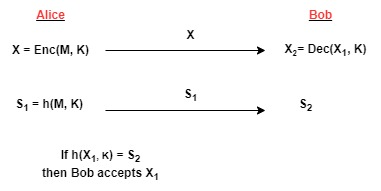
\includegraphics[width=8cm]{Hash1.jpg}
	\end{center}
	\subsection{Definition}
	A Hash function is a four tuple (P, S, K, H) where the following conditions are satisfied 
	\begin{enumerate}
		\item P is the set of all possible messages.
		\item S is the set of all possible message digests or authentication tags.
		\item K is the key space
		\item For each K\textsubscript{i} $\in$ K there is a hash function h\textsubscript{K\textsubscript{i}} $\in$ H such that\\
		h\textsubscript{K\textsubscript{i}} : P $\rightarrow$ S
	\end{enumerate}
	Here $|$P$|$ $\geq$ $|$S$|$\\
	More interestingly $|$P$|$ $\geq$ 2$\ast|$S$|$\\
	\begin{center}
		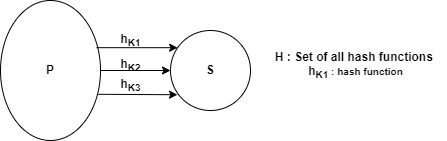
\includegraphics[width=10cm]{Hash2.jpg}
	\end{center}
	$\bullet$ If key is involved in the computation of hashed valve then the hash function is known as keyed hash function.\\
	$\bullet$ If key is not required to compute the hashed valve then the hash function is known as unkeyed hash function.
	\section{Problems}
	\subsection{Problem 01}
	h : P $\rightarrow$ S\\
	Given y $\in$ S Find x $\in$ P\\
	such that h(x) = y\\
	This problem is known as pre-image finding problem.\\
	For an hash function h if you cannot find pre-image in a feasible time then h is known as pre-image resistant hash function.\\
	$\bullet$ Finding pre-image is computationally hard for pre-image resistant hash function.
	\subsection{Problem 02}
	h : P $\rightarrow$ S\\
	Given x $\in$ P and h(x) find x$^l$ $\in$ P such that x$^l$ $\neq$ x and h(x$^l$) = h(x).\\
	This problem is known as second pre-image finding problem.\\
	If finding second pre-image is computationally hard for h then h is known as second pre-image resistant hash function.
	\subsection{Problem 03}
	h : P $\rightarrow$ S\\
	Find x, x$^l$ $\in$ P such that x $\neq$ x$^l$ and h(x) = h(x$^l$)\\
	This problem is known as collision finding problem.\\
	If finding collision is computationally hard then h is known as collision resistant hash function.
	\subsection*{Ideal Hash Function}
	Let h : P $\rightarrow$ S be an hash function.\\h will be called ideal hash function if given x $\in$ P to find h(x) either you have to apply h on x or you have to look into the table corresponding to h (hash table).
	\section{Pre Image Finding Problem Algorithm}
	h : X $\rightarrow$ Y\\
	$|$X$|$ = n and $|$Y$|$ = m\\
	Y = \{y\textsubscript{1}, y\textsubscript{2},..., y\textsubscript{m}\}\\
	X\textsubscript{0} $\subseteq$ X, $|$X\textsubscript{0}$|$ = Q.\\
	\hspace*{0.8cm}for each x $\in$ X\textsubscript{0}\\
	\hspace*{1.3cm}compute y\textsubscript{x} = h(x)\\
	\hspace*{1.3cm}if y\textsubscript{x} = y\\
	\hspace*{1.3cm}return x\\
	E\textsubscript{i} = event h(x\textsubscript{i}) = y, 1 $\leq$ i $\leq$ Q.\\
	Pr[E\textsubscript{i}] = 1/M\\
	Pr[E\textsubscript{i}$^c$] = 1 - 1/M\vspace{0.1cm}\\
	Pr[E\textsubscript{1} $\cup$ E\textsubscript{2} $\cup$... $\cup$ E\textsubscript{Q}] \\
	= 1 - Pr[E\textsubscript{1}$^c$ $\cap$ E\textsubscript{2}$^c$ $\cap$... $\cap$ E\textsubscript{Q}$^c$]\hfill 
	\begin{tabular}{| c |}
		\hline
		Since every event is independent of other\\
		\hline
	\end{tabular}\vspace{0.1cm}\\
	= 1 - Pr[E\textsubscript{1}$^c$]$\ast$Pr[E\textsubscript{2}$^c$]$\ast$...$\ast$Pr[E\textsubscript{Q}$^c$]\hfill 
	\begin{tabular}{| c |}
		\hline
		If A \& B are independent Pr[A $\cap$ B] = Pr[A] $\ast$ Pr[B]\\
		\hline
	\end{tabular}\\
	= 1 - $\Pi$(Pr[E\textsubscript{i}$^c$])\\
	= 1 - [1 - $\frac{1}{M}$]$^Q$\\
	= 1 - [1 - $(\frac{Q}{1})\frac{1}{M}$ +  $(\frac{Q}{2})\frac{1}{M^2}$ +  $(\frac{Q}{3})\frac{1}{M^3}$ + ...]\\
	= 1 - (1 -  $\frac{Q}{M}$) \hfill 
	\begin{tabular}{| c |}
		\hline
		Since M $>>$ 1\\
		\hline
	\end{tabular}\\
	= 1 - 1 +  $\frac{Q}{M}$\\
	= $\frac{Q}{M}$\\
	Complexity = $\frac{1}{Probability}$ = $\frac{1}{\frac{Q}{M}}$\\
	$\therefore$ Complexity = $\frac{M}{Q}$ = O(M)
	
\end{document}